% questions.tex —— 2006 年·普通高等学校招生考试·辽宁卷文科 · 题目内容片段（无答案）
% 由 tools/generate_projects.py 依来源总账自 2006/2006_数学真题_辽宁文_试题.md 生成，勿手改（改源 MD 后重跑）


\begin{gktip}
\textbf{来源边界}：据固定候选 PDF 逐题转录，SHA-256 与 source manifest 记录一致。题签与源页支持卷名和科类，但不能认证发布者、出版者、版次、扫描/重排来源链或官方原件身份。固定 PDF 未见答案、解析或评分标准，官方答案未录入。

\textbf{源页定位}：PDF 第 1 页（印刷页 310）含 Q1–Q19；第 2 页（印刷页 311）含 Q20–Q22。选择题 Q1–Q12，填空题 Q13–Q16，解答题 Q17–Q22。

\textbf{转录说明}：按原页保留题意、符号和选项，不依推测补写或纠错。Q15、Q19 图稿已按固定源结构矢量重绘，坐标不表示比例。

\textbf{原文存疑}：Q21（2）原页印作“四边形 APCD”，但前文定义的点依次为 A、B、C、D；保留原字样 P，不推测改成 ABCD，待来源问题登记后再处理。
\end{gktip}

\gkpart{一、选择题}

\begin{question}
\gkti{1}
\Needspace{5\baselineskip}
函数
\nopagebreak[4]
\[
y=\sin\left(\frac12x+3\right)
\]
的最小正周期是（ ）。

(A) \(\frac{\pi}{2}\)　(B) \(\pi\)　(C) \(2\pi\)　(D) \(4\pi\)

\end{question}
\begin{question}
\gkti{2}
设集合 \(A=\{1,2\}\)，则满足 \(A\cup B=\{1,2,3\}\) 的集合 \(B\) 的个数是（ ）。

(A) 1　(B) 3　(C) 4　(D) 8

\end{question}
\begin{question}
\gkti{3}
设 \(f(x)\) 是 \(\mathbb R\) 上的任意函数，则下列叙述正确的是（ ）。

(A) \(f(x)f(-x)\) 是奇函数

(B) \(f(x)|f(-x)|\) 是奇函数

(C) \(f(x)+f(-x)\) 是偶函数

(D) \(f(x)-f(-x)\) 是偶函数

\end{question}
\begin{question}
\gkti{4}
\nopagebreak[4]
\[
C_6^1+C_6^2+C_6^3+C_6^4+C_6^5
\]
的值为（ ）。

(A) 61　(B) 62　(C) 63　(D) 64

\end{question}
\begin{question}
\gkti{5}
方程 \(2x^2-5x+2=0\) 的两个根可分别作为（ ）。

(A) 一个椭圆和一双曲线的离心率

(B) 两抛物线的离心率

(C) 一个椭圆和一抛物线的离心率

(D) 两椭圆的离心率

\end{question}
\begin{question}
\gkti{6}
给出下列四个命题：

① 垂直于同一直线的两条直线互相平行；

② 垂直于同一平面的两个平面互相平行；

③ 若直线 \(l_1,l_2\) 与同一平面所成的角相等，则 \(l_1,l_2\) 互相平行；

④ 若直线 \(l_1,l_2\) 是异面直线，则与 \(l_1,l_2\) 都相交的两条直线是异面直线。

其中假命题的个数是（ ）。

(A) 1　(B) 2　(C) 3　(D) 4

\end{question}
\begin{question}
\gkti{7}
双曲线 \(x^2-y^2=4\) 的两条渐近线与直线 \(x=3\) 围成一个三角形区域，表示该区域的不等式组是（ ）。

(A) \(\begin{cases}x-y\ge 0,\\x+y\ge 0,\\0\le x\le 3.\end{cases}\)

(B) \(\begin{cases}x-y\ge 0,\\x+y\le 0,\\0\le x\le 3.\end{cases}\)

(C) \(\begin{cases}x-y\le 0,\\x+y\le 0,\\0\le x\le 3.\end{cases}\)

(D) \(\begin{cases}x-y\le 0,\\x+y\ge 3,\\0\le x\le 3.\end{cases}\)

\end{question}
\begin{question}
\gkti{8}
设 \(\oplus\) 是 \(\mathbb R\) 上的一个运算，\(A\) 是 \(\mathbb R\) 的非空子集，若对任意 \(a,b\in A\)，有 \(a\oplus b\in A\)，则称 \(A\) 对运算 \(\oplus\) 封闭。下列数集对加法、减法、乘法和除法（除数不等于零）四则运算都封闭的是（ ）。

(A) 自然数集　(B) 整数集　(C) 有理数集　(D) 无理数集

\end{question}
\begin{question}
\gkti{9}
\Needspace{5\baselineskip}
\(\triangle ABC\) 的三内角 \(A,B,C\)，所对边的长分别为 \(a,b,c\)。设向量
\nopagebreak[4]
\[
\vec p=(a+c,b),\qquad \vec q=(b-a,c-a).
\]
若 \(\vec p\parallel\vec q\)，则角 \(C\) 的大小为（ ）。

(A) \(\frac\pi6\)　(B) \(\frac\pi3\)　(C) \(\frac\pi2\)　(D) \(\frac{2\pi}3\)

\end{question}
\begin{question}
\gkti{10}
已知等腰 \(\triangle ABC\) 的腰为底的 2 倍，则顶角 \(A\) 的正切值是（ ）。

(A) \(\frac{\sqrt3}{2}\)　(B) \(\sqrt3\)　(C) \(\frac{\sqrt{15}}8\)　(D) \(\frac{\sqrt{15}}7\)

\end{question}
\begin{question}
\gkti{11}
\Needspace{5\baselineskip}
与方程
\nopagebreak[4]
\[
y=e^{2x}-2e^x+1\quad (x\ge 0)
\]
的曲线关于直线 \(y=x\) 对称的曲线方程为（ ）。

(A) \(y=\ln(1+\sqrt{x})\)　(B) \(y=\ln(1-\sqrt{x})\)

(C) \(y=-\ln(1+\sqrt{x})\)　(D) \(y=-\ln(1-\sqrt{x})\)

\end{question}
\begin{question}
\gkti{12}
\Needspace{5\baselineskip}
曲线
\nopagebreak[4]
\[
\frac{x^2}{10-m}+\frac{y^2}{6-m}=1\quad(m<6)
\]
\Needspace{5\baselineskip}
与曲线
\nopagebreak[4]
\[
\frac{x^2}{5-n}+\frac{y^2}{9-n}=1\quad(5<n<9)
\]
的（ ）。

(A) 离心率相等　(B) 焦距相等　(C) 焦点相同　(D) 准线相同

\end{question}
\gkpart{二、填空题}

\begin{question}
\gkti{13}
\Needspace{5\baselineskip}
方程
\nopagebreak[4]
\[
\log_2(x-1)=2-\log_2(x+1)
\]
的解为 \gkblank{}。

\end{question}
\begin{question}
\gkti{14}
\Needspace{5\baselineskip}
设
\nopagebreak[4]
\[
g(x)=\begin{cases}e^x,&x\le 0,\\\ln x,&x>0,\end{cases}
\]
则 \(g\left(g\left(\frac12\right)\right)=\) \gkblank{}。

\Needspace{0.4\textheight}
\end{question}
\begin{question}
\gkti{15}
如图，半径为 2 的半球内有一内接正六棱锥 \(P-ABCDEF\)，则此正六棱锥的侧面积是 \gkblank{}。
\nopagebreak[4]
\begin{center}% Generator: hand-authored TikZ schematic; coordinates are not to scale.
% Source: fixed 2006 Liaoning arts candidate PDF, source ID
% src-b784613ebc50375b17eb4a91083b447879ebb9ed75bb6a76227bb74345cfbfd3,
% SHA-256 bbb83af465d4650c594f23a879d82dea43a86f805b6fc8712d25809aac7fda22,
% PDF page 1, printed page 310, Q15.
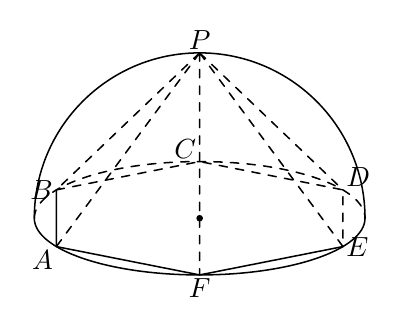
\begin{tikzpicture}[line cap=round,line join=round,line width=0.55pt]
  % Schematic perspective of the hemisphere and the inscribed regular hexagon.
  \coordinate (P) at (0,2.70);
  \coordinate (A) at (-1.82,0.24);
  \coordinate (B) at (-1.82,0.96);
  \coordinate (C) at (0,1.32);
  \coordinate (D) at (1.82,0.96);
  \coordinate (E) at (1.82,0.24);
  \coordinate (F) at (0,-0.12);

  % Outer profile of the hemisphere and its equatorial rim.
  \begin{scope}[shift={(0,0.60)}]
    \draw (-2.10,0) arc (180:0:2.10);
    \draw[dashed] (-2.10,0) arc (180:0:2.10 and 0.72);
    \draw (2.10,0) arc (0:-180:2.10 and 0.72);
  \end{scope}

  % Hidden rear edges of the base hexagon and all pyramid edges inside the dome.
  \draw[dashed] (B)--(C)--(D)--(E);
  \draw[dashed] (P)--(A) (P)--(B) (P)--(C) (P)--(D) (P)--(E) (P)--(F);
  % Visible front edges of the base hexagon.
  \draw (E)--(F)--(A)--(B);

  % Unlabelled center mark shown in the source diagram.
  \fill (0,0.60) circle (1.2pt);
  \node[above,inner sep=1pt] at (P) {$P$};
  \node[below left,inner sep=1pt] at (A) {$A$};
  \node[left,inner sep=1pt] at (B) {$B$};
  \node[above left,inner sep=1pt] at (C) {$C$};
  \node[above right,inner sep=1pt] at (D) {$D$};
  \node[right,inner sep=1pt] at (E) {$E$};
  \node[below,inner sep=1pt] at (F) {$F$};
\end{tikzpicture}
\end{center}
\nopagebreak[4]
\end{question}
\begin{question}
\gkti{16}
5 名乒乓球队员中，有 2 名老队员和 3 名新队员。现从中选出 3 名队员排成 1、2、3 号参加团体比赛，则入选的 3 名队员中至少有 1 名老队员，且 1、2 号中至少有 1 名新队员的排列方法有 \gkblank{} 种。（以数作答）

\end{question}
\gkpart{三、解答题}

\begin{question}
\gkti{17}
\Needspace{5\baselineskip}
已知函数
\nopagebreak[4]
\[
f(x)=\sin^2x+2\sin x\cos x+3\cos^2x,\qquad x\in\mathbb R.
\]
求：

(1) 函数 \(f(x)\) 的最大值及取得最大值的自变量 \(x\) 的集合；

(2) 函数 \(f(x)\) 的单调增区间。

\end{question}
\begin{question}
\gkti{18}
甲、乙两班各派 2 名同学参加年级数学竞赛，参赛同学成绩及格的概率都为 0.6，且参赛同学的成绩相互之间没有影响。求：

(1) 甲、乙两班参赛同学中各有 1 名同学成绩及格的概率；

(2) 甲、乙两班参赛同学中至少有 1 名同学成绩及格的概率。

\Needspace{0.4\textheight}
\end{question}
\begin{question}
\gkti{19}
已知正方形 \(ABCD\)，\(E、F\) 分别是边 \(AB、CD\) 的中点，将 \(\triangle ADE\) 沿 \(DE\) 折起，如图所示，记二面角 \(A-DE-C\) 的大小为 \(\theta\)（\(0<\theta<\pi\)）。

(1) 证明：\(BF\parallel\) 平面 \(ADE\)；

(2) 若 \(\triangle ACD\) 为正三角形，试判断点 \(A\) 在平面 \(BCDE\) 内的射影 \(G\) 是否在直线 \(EF\) 上，证明你的结论，并求角 \(\theta\) 的余弦值。
\nopagebreak[4]
\begin{center}% Generator: hand-authored TikZ schematic; coordinates are not to scale.
% Source: fixed 2006 Liaoning arts candidate PDF, source ID
% src-b784613ebc50375b17eb4a91083b447879ebb9ed75bb6a76227bb74345cfbfd3,
% SHA-256 bbb83af465d4650c594f23a879d82dea43a86f805b6fc8712d25809aac7fda22,
% PDF page 1, printed page 310, Q19.
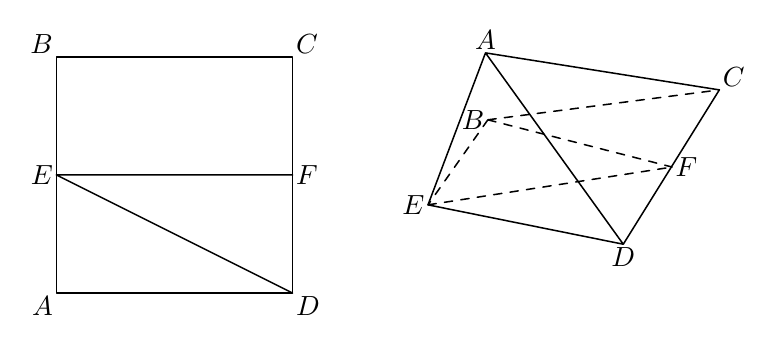
\begin{tikzpicture}[line cap=round,line join=round,line width=0.55pt]
  % Flat square before folding; E and F are the midpoints of AB and CD.
  \coordinate (A0) at (0,0);
  \coordinate (B0) at (0,3);
  \coordinate (C0) at (3,3);
  \coordinate (D0) at (3,0);
  \coordinate (E0) at (0,1.5);
  \coordinate (F0) at (3,1.5);
  \draw (A0)--(B0)--(C0)--(D0)--cycle;
  \draw (E0)--(F0) (E0)--(D0);
  \node[below left,inner sep=1pt] at (A0) {$A$};
  \node[above left,inner sep=1pt] at (B0) {$B$};
  \node[above right,inner sep=1pt] at (C0) {$C$};
  \node[below right,inner sep=1pt] at (D0) {$D$};
  \node[left,inner sep=1pt] at (E0) {$E$};
  \node[right,inner sep=1pt] at (F0) {$F$};

  % Folded view: BCDE is the fixed plane; triangle ADE is rotated about DE.
  % AC is drawn because part (2) explicitly invokes triangle ACD.
  \coordinate (A) at (5.45,3.05);
  \coordinate (B) at (5.48,2.20);
  \coordinate (C) at (8.42,2.58);
  \coordinate (D) at (7.20,0.62);
  \coordinate (E) at (4.72,1.12);
  \coordinate (F) at (7.82,1.60);
  \draw[dashed] (B)--(C) (B)--(E) (B)--(F) (E)--(F);
  \draw (C)--(D)--(E) (A)--(E) (A)--(D) (A)--(C);
  \node[above,inner sep=1pt] at (A) {$A$};
  \node[left,inner sep=1pt] at (B) {$B$};
  \node[above right,inner sep=1pt] at (C) {$C$};
  \node[below,inner sep=1pt] at (D) {$D$};
  \node[left,inner sep=1pt] at (E) {$E$};
  \node[right,inner sep=1pt] at (F) {$F$};
\end{tikzpicture}
\end{center}
\nopagebreak[4]
\end{question}
\begin{question}
\gkti{20}
\Needspace{5\baselineskip}
已知等差数列 \(\{a_n\}\) 的前 \(n\) 项和为
\nopagebreak[4]
\[
S_n=pn^2-2n+q\quad(p,q\in\mathbb R),\qquad n\in\mathbb N^+.
\]

(1) 求 \(q\) 的值；

(2) 若 \(a_1\) 与 \(a_5\) 的等差中项为 18，\(b_n\) 满足 \(a_n=2\log_2b_n\)，求数列 \(\{b_n\}\) 的前 \(n\) 项和。

\end{question}
\begin{question}
\gkti{21}
\Needspace{5\baselineskip}
已知函数
\nopagebreak[4]
\[
f(x)=\frac13ax^3+(a+d)x^2+(a+2d)x+d,\qquad
g(x)=ax^2+2(a+2d)x+a+4d,
\]
\Needspace{5\baselineskip}
其中 \(a>0,d>0\)。设 \(x_0\) 为 \(f(x)\) 的极小值点，\(x_1\) 为 \(g(x)\) 的极值点，\(g(x_2)=g(x_3)=0\)，并且 \(x_2<x_3\)。将点
\nopagebreak[4]
\[
(x_0,f(x_0)),\ (x_1,g(x_1)),\ (x_2,0),\ (x_3,0)
\]
依次记为 \(A,B,C,D\)。

(1) 求 \(x_0\) 的值；

(2) 若四边形 \(APCD\) 为梯形且面积为 1，求 \(a,d\) 的值。

\end{question}
\begin{question}
\gkti{22}
\Needspace{5\baselineskip}
已知点 \(A(x_1,y_1)、B(x_2,y_2)\)（\(x_1,x_2\ne0\)）是抛物线
\nopagebreak[4]
\[
y^2=2px\quad(p>0)
\]
\Needspace{5\baselineskip}
上的两个动点，\(O\) 是坐标原点，向量 \(\overrightarrow{OA},\overrightarrow{OB}\) 满足
\nopagebreak[4]
\[
\left|\overrightarrow{OA}+\overrightarrow{OB}\right|=
\left|\overrightarrow{OA}-\overrightarrow{OB}\right|.
\]
\Needspace{5\baselineskip}
设圆 \(C\) 的方程为
\nopagebreak[4]
\[
x^2+y^2-(x_1+x_2)x-(y_1+y_2)y=0.
\]

(1) 证明线段 \(AB\) 是圆 \(C\) 的直径；

(2) 当圆 \(C\) 的圆心到直线 \(x-2y=0\) 的距离的最小值为 \(\frac{2\sqrt5}{5}\) 时，求 \(p\) 的值。

\end{question}